\chapter{Overall Description}

\section{Product Perspective}
The image~\ref{figure:UML} shows the mock-up of the system made in \gls{uml}. The \gls{uml} is not definitive model, but it shows the starting point of the \gls{clup} system. It is made to help visualize the main elements of our system and their interactions. The scheme wants to highlight the following interactions:
\begin{itemize}

	\item The ticket represents the person inside the queue.

	\item The physical spot is treated like a user in the system, the default one. 

	\item Since the booking ticket may point to different days, they are not immediately saved in the queue but instead in a booking list that will interact with the 	queue to schedule at the right time.

	\item The dashboard interacts with the system elements to show relevant data. 
\end{itemize}

\begin{figure}[H]
	\centering
	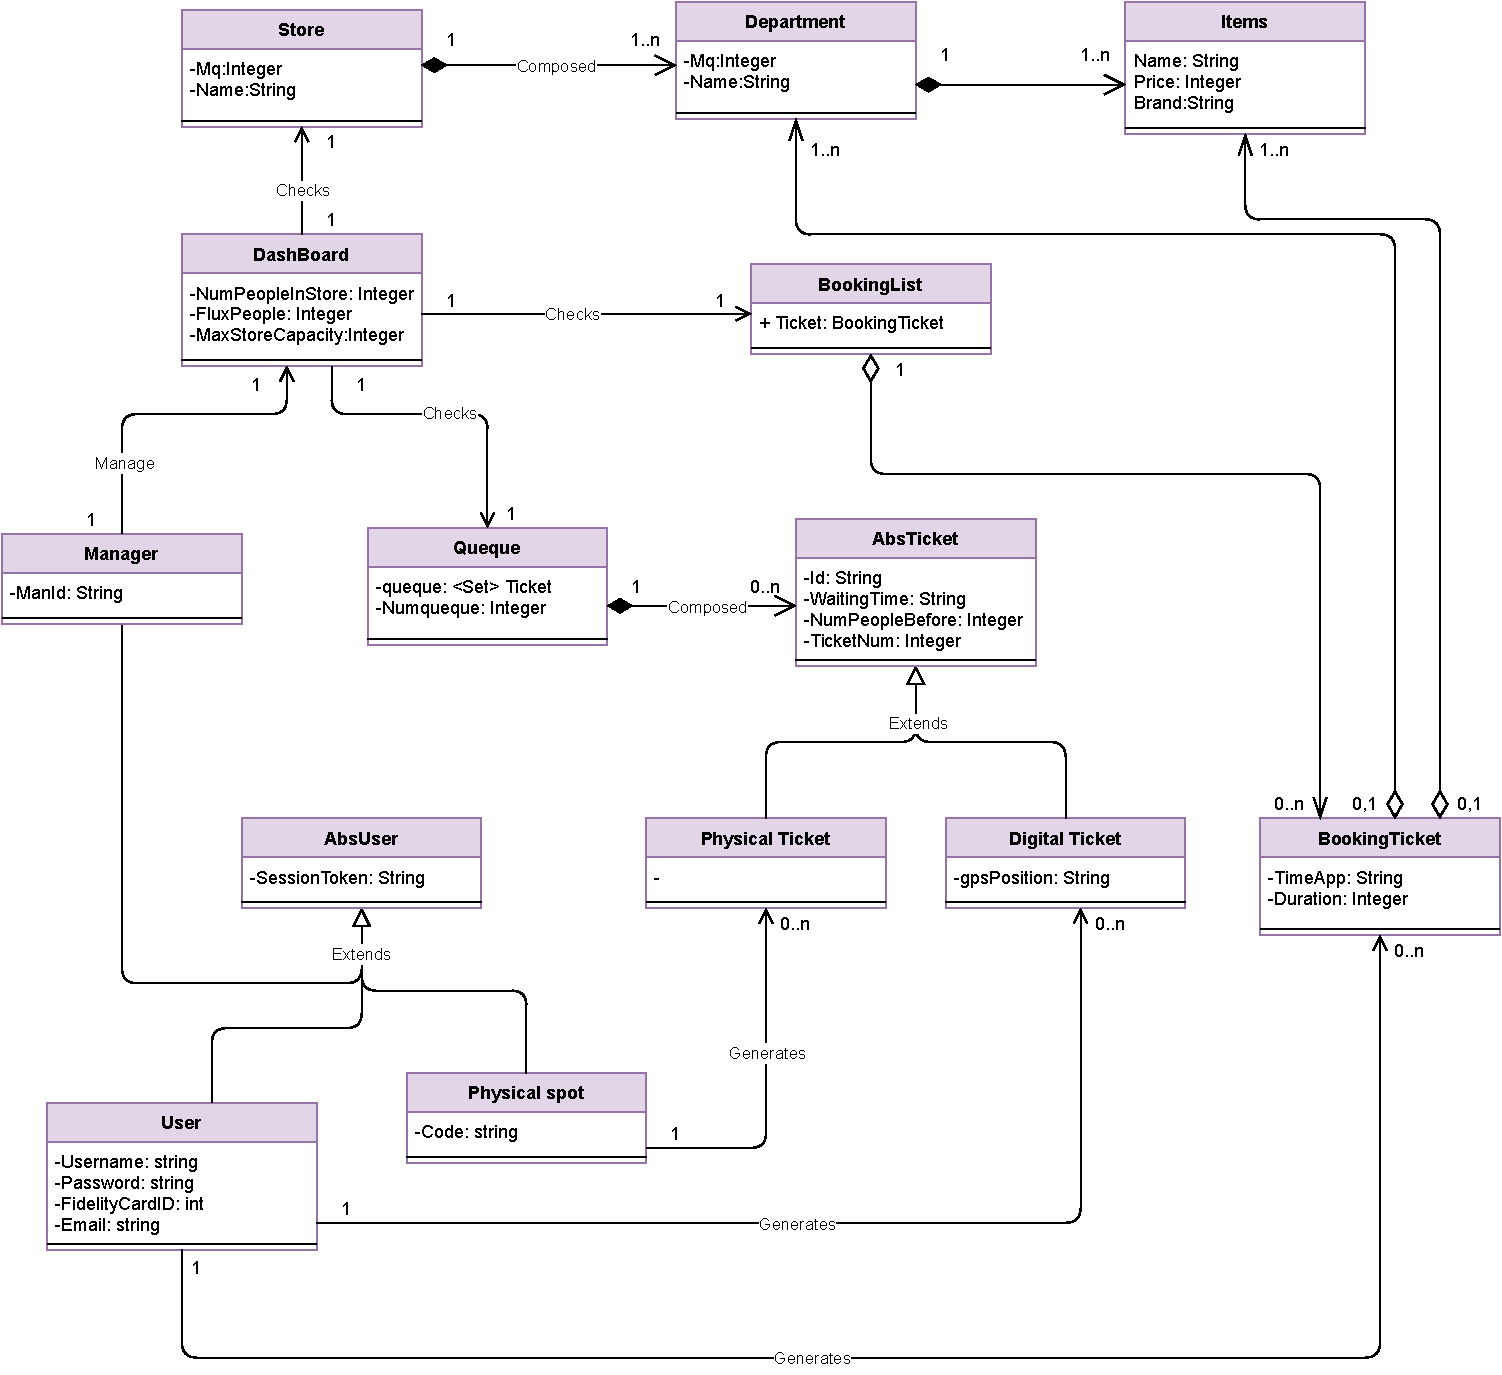
\includegraphics[width=1.0\textwidth]{images/UML.pdf}
	\caption{Class diagram.}
	\label{figure:UML}
\end{figure}

In the next state diagrams, it will be shown how the lining up feature works. It will also highlight the difference in the handling between the physical ticket and the digital ticket.


\begin{figure}[H]
	\centering
	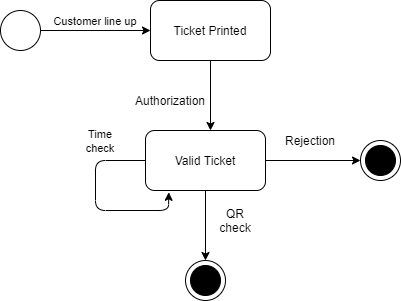
\includegraphics[scale = 0.5]{images/TicketPhysical.png}
	\caption{State diagram physical ticket.}
\end{figure}


\begin{figure}[H]
	\centering
	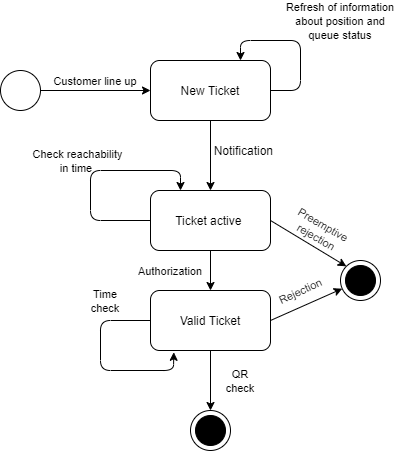
\includegraphics[scale = 0.5]{images/statechart.png}
	\caption{State diagram digital ticket.}
\end{figure}

The main difference is that in the digital lining up, since it can be done from a distant position, \gls{clup} must first calculate a feasible time to reach the store and then schedule it in the queue. Instead, the physical lining up it is immediately scheduled since the position is the store one. The second difference is that for the digital lining up a notification is sent to the customer, that suggest going to the store when it is the right time. It is possible that other notifications are sent, if the reachable time check is violated, and if it exceeds a certain value the ticket is preemptively discarded. Instead for the physical one, since they are close to the store and that is not possible to notify them, they will able only to wait.
The end is the same for both, the ticket will authorize them to enter for a period then if not used it will expire.


\section{Product Functions}

In this section are described the main functionalities offered by the service.

\subsection{Lining Up}
In light of the motivations described in the previous sections, the main purpose of the application is to allow customers to line up from remote.\\
To achieve this result, the application provides the possibility to line up from the smartphone.
The users have to log in the application, select the lining up operation, choose the store (in which they want to go) and confirm.
Once the operation has been completed successfully, users are able to check the status of the queue and watch the QR code associated to the lining up.
Moreover, users will receive live notifications about the status and the remaining time to be authorized to enter in the store.
When the countdown is ending, customers have to approach to the store and wait outside for the call of their ticket number (showed with the QR code). At this time, they have to show the QR code to be scanned by the system and to be authorized to enter.

From the point of view of the server, when it receives the request, it has to check if the user can be allocated in the virtual queue and in which position. If it can, the user will be allocated, otherwise it will reply with an error message.
The application sends to the server information about the global position of the customer. These information are used to estimate the time necessary by the customer to arrive to the store.
All the collected information are used to schedule the entrances to the store.
More precisely, the algorithm takes into account the position of the customer, to infer the cruise speed and the time needed to arrive, the number of customers already inside the store, the number of customers previously allocated to the virtual queue and the number of customers in the physical queue.
The server can infer the residence time in the store looking at previous purchases of the same user or by computing the average residence time of the customers.
Based on these data, the order in which customers ask for a lining up operation can be different by the allocation order in the virtual queue. In case of huge delays (parameter that can be controlled by the store manager) by the customers, the virtual queue can be reorganized dynamically.

\subsection{Booking a Visit}
This functionality is an extension of the previous one, in particular it allows to specify the date and time to visit the store.\\
To book a visit, customers should select the corresponding button from the menu of the application, insert the requested data, such as the store in which they want to go, the date, the slot time, the category of grocery they want to buy (it is not mandatory), and confirm the operation.
As for the lining up operation, customers can check the status and the obtained QR code.

From the point of view of the server, the behavior is similar to the lining up, but in this case it can infer more information from the category of grocery specified, such as the section in the store that will be visited by the customer. If not specified, the server can infer information from previous purchases.
In any case, the server can allocate users in a finer way in the virtual queue exploiting these data: knowing the maximum capacity of the store and the section with higher density of customers, it can decide if an user has to be allocated in one or another time slot.

\subsection{Lining Up from Physical Spot}
If a customer hasn't an user account, or if he doesn't want to use (or can't use) the smartphone application, he can line up from a physical spot installed outside the store.
The physical spot is a digital device that runs the same smartphone application used by other users, but with less functionalities.
From the physical spot, a customer can line up clicking on a button to confirm the operation and the spot will print the ticket showing the QR code and the ticket number.

The physical spot acts as proxy. The physical spot is logged in the application with a custom account. In this way customers haven't to insert the credentials when they perform a lining up operation.
The server retrieves the missing information (destination store, position of the customer, etc.), about the lining up, by the association between the physical spot account and the associated store (It can be best appreciated in ~\ref{figure:liningUpSequenceDiagram}).
In this way the physical spot can be treated as a common user.

\subsection{Monitoring and Controlling the Queue}
These are functionalities dedicated to the store manager. Since the system performs different estimations, it can occur that the real situation differs from the theorized sequence of events.
To handle this possibility, the store manager can monitor the status of the queue and the number of customers inside and outside the store from his device and decide if the server has to schedule in a different way the users arrivals.
To do that, the application provides a different home page, if you are logged in with a store manger account, that provides buttons and interfaces to get the status of the situation and to set scheduling parameters that the server will use. In extreme cases he can stop issuing tickets.

% TODO: inserisco qua la questione del tornello connesso al dispositivo del manager?

\section{User Characteristics}

The actors in our application are the following:

\begin{itemize}

	\item Customer: is a person who has downloaded the application and regularly uses it to interact with the store. The first time they use it, they have to register. The following times they must log in and authenticate in order to use the functionality of the application. Then they can either line up remotely or book a visit. If they uses the line-up function, then, for some time they can view the relative ticket with the associated data. Same happens
	when using the function of booking a visit, after compiling the form and sending it, they can look at their appointments data for a period.
	\item Physical spot: represents users that do not have the application and gives them the possibility to use the line-up function. It does that by handing to them a paper ticket which represent a position in the digital queue.
	\item Store manager: is the person responsible of the store, and the one who can log as manager in the application.They are given a dashboard where they can check relevant data regarding the store, the influx of the people in it and the status of the queue. They can modify parameters important to the elaborations of the data and take decisions that influence the influx of people, like stopping the release of new tickets for a time period. 

\end{itemize}

\section{Assumptions, Dependencies and Constraints}

Below, the list of our domain assumptions has been reported.

\begin{itemize}

	\item \textbf{{[D1]}}: There is a \gls{dpcm} in force.
	\item \textbf{{[D2]}}: Customers follow the rules imposed by the \gls{dpcm} in force.
	\item \textbf{{[D3]}}: Customers enter in the store only if the system authorizes them.
	\item \textbf{{[D4]}}: Customers don't stay in the shop longer than necessary and they go away from the store after they have done their shopping.
	\item \textbf{{[D5]}}: Customers line up physically only if they have a valid (non expired) QR code.
	\item \textbf{{[D6]}}: Outside the store there is space to queue.
	\item \textbf{{[D7]}}: Customers have a smartphone.
	\item \textbf{{[D8]}}: Customers have installed the \gls{clup} application.
	\item \textbf{{[D9]}}: Users allow the permissions requested by the application.
	\item \textbf{{[D10]}}: Users keep Internet connection active.
	\item \textbf{{[D11]}}: There is a store manager present in the store.
	\item \textbf{{[D12]}}: Physical spots are powered on every working day.
	\item \textbf{{[D13]}}: Physical spots are refilled when asked by the system.

\end{itemize}